\section{Objetives}

The purpose of this laboratory session is to mechanically characterize different
types of composites materials by using normalized tensile testing.\\

\section{Materials}

The materials used for this session were three types of thermoplastic composites.\\

\subsection{Virgin polypropilene (uPP)}

First of all we are testing the matrix base itself, without any reinforcement fibers.
The Polypropliene is material solid, ductile and flexible at room temperature.

In order to perform the tests, the thermoplastic was melted over its melting
point, 165ºC, and injected into two molds prepared for the tensile testing.\\

\begin{figure}[h]
	\centering
	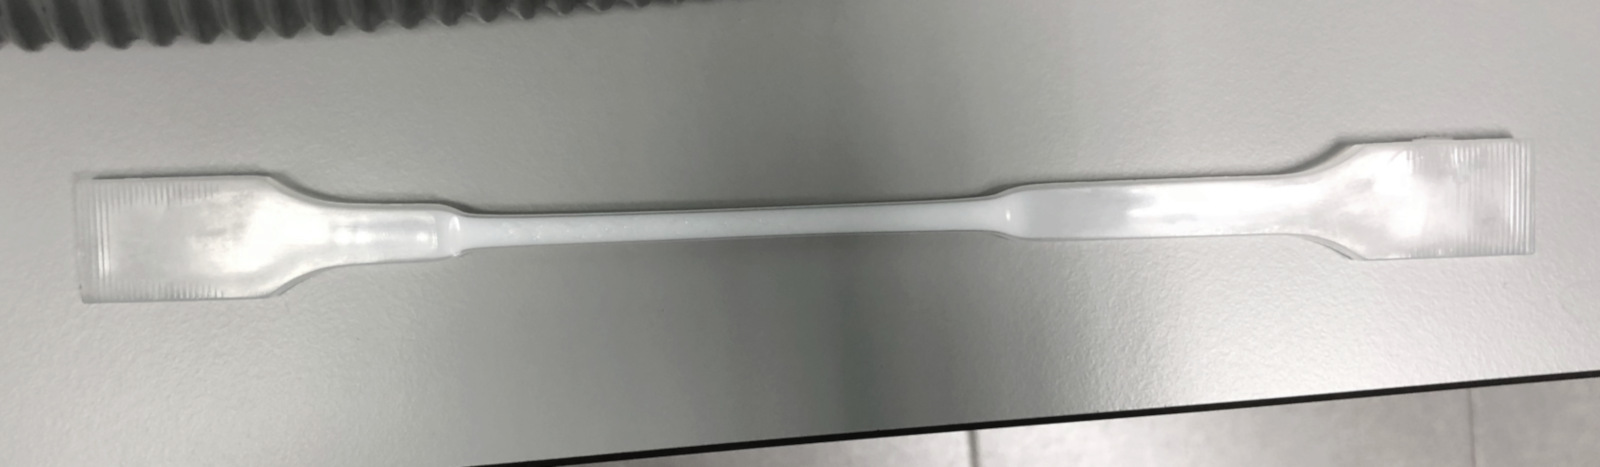
\includegraphics[width=0.8\textwidth]{img/1_Unreinforced_PP.jpg}
	\caption[short caption]{Unreinforced PP sample after test}
	\label{fig:unreinforced_PP}
\end{figure}

\subsection{Polypropliene with 30\% weight short glass fibers}

As a second material to be tested we used the same polypropilene matrix but mixed
with 30\% in weight short glass fibers, of about 4mm long. The preceodure to create
the sample to be tested is similar. Melting the PP, join the glass fibers and mix
all together, and inject it inside the mold.\\

\begin{figure}[h]
	\centering
	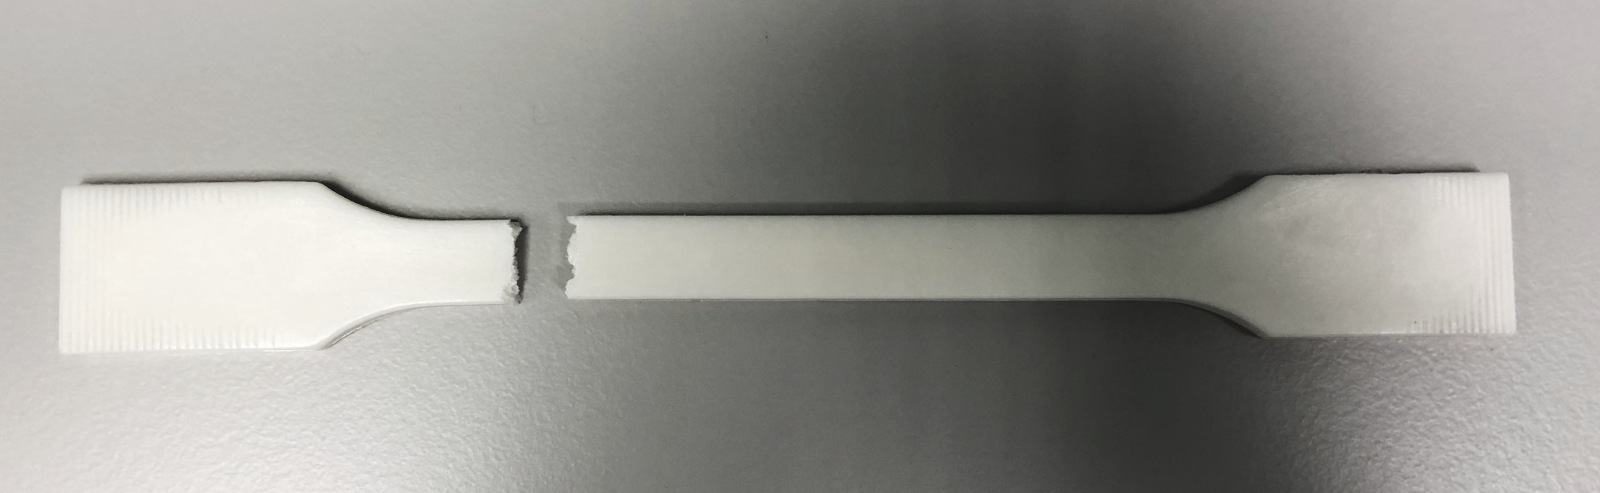
\includegraphics[width=0.8\textwidth]{img/2_PP_short_glass_fibre.jpg}
	\caption[short caption]{PP reinforced with 30\% weight short glass fibers}
	\label{fig:PP30}
\end{figure}

\subsection{Polypropliene with continous fibers}

In this case, the polypropilene base impregnate a continuos glass fiber fabric.
The material used in this practice has the commercial name of Twintex\textsuperscript{\tiny\textregistered}
and is made of polypropilene with a continuous glass fiber structure which constitute
the 60\% in weight. As the material could be anisotropic regarding the manufacturing
direcction, the test were performed in both transversal and machine direction.\\

\begin{figure}[h]
	\centering
	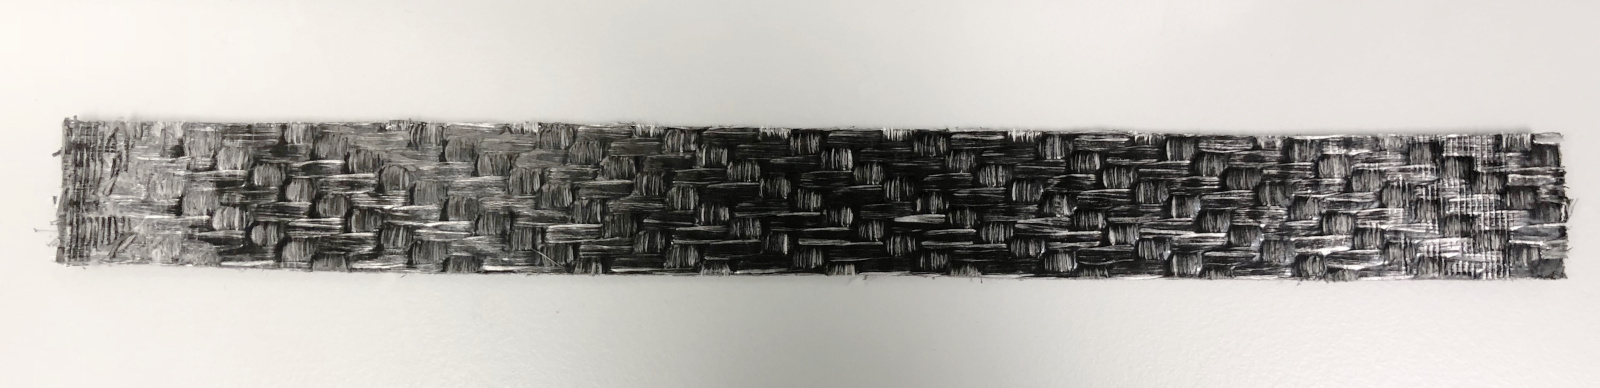
\includegraphics[width=0.8\textwidth]{img/3_Twintex.jpg}
	\caption[short caption]{Twintex}
	\label{fig:twintex}
\end{figure}

In every case, the way of measuring the mass fiber fraction consists in burning
the material, so the organic part, the plastic, burns out, leaving just the
inorganic part, the glass fiber. Weighting the material before and after, we can
obtain the mass-fraction of fibers present in the sample.\\

\section{Equipment and machinery}

It was used an universal testing machine, tensile tester, which was able to perform
a deformation at a constant velocity and record the load required to maintain this
constant velocity.\\

The maximum load that the equipment supports is 10kN, so in case of reaching this
values during the experiment, the test must be stopped to avoid damaging the sensor
or the machine.\\


\section{Experimental procedure}

During the experimental session a series of procedures was performed for every
sample previously mentioned.\\

\begin{enumerate}
	\item The laminated thermoset-based polymer composites is placed in the
	testing machine grabbed by the clamps and secured with the screws of each clamp.
	\item We turn the machine on under a constant movement of the superior
	clamp of 10 mm/s
	\item Once it breaks or when we consider it is enough time for having
	optimal results, the machine is turned off, the clamps opened and the
	laminated thermoset-based polymer composite is removed.
	\item Repeat steps above for the thermoplastic-based polymer composite.
\end{enumerate}

\section{Results and discussion}



\section{Conclusion}
